\documentclass[11pt,reqno]{amsart}
\usepackage[margin=1.5in]{geometry}                % See geometry.pdf to learn the layout options. There are lots.
\geometry{letterpaper}                   % ... or a4paper or a5paper or ... 
%\geometry{landscape}                % Activate for for rotated page geometry
%\usepackage[parfill]{parskip}    % Activate to begin paragraphs with an empty line rather than an indent
\usepackage{amsmath}
\usepackage{amsfonts}
\usepackage{amssymb}
\usepackage{mathrsfs}%Ralph Smith's Formal Script font
\usepackage[retainorgcmds]{IEEEtrantools}%IEEEeqnarray environment
\usepackage{graphicx}%import graphics
\usepackage{subfigure}%subfigures
\usepackage{listings}
\usepackage[font=small]{caption}
\usepackage[usenames,dvipsnames]{color}
\usepackage{amsthm}
\DeclareGraphicsRule{.tif}{png}{.png}{`convert #1 `dirname #1`/`basename #1 .tif`.png}

%%set margins:
%\topmargin=-0.45in      
%\evensidemargin=0in     
%\oddsidemargin=0in      
%\textwidth=6.5in        
%\textheight=9in  

%%%%%%%%%%%%%%%%%%%%%%%%%%%%%%%%%%%%%%%%%%

\mathchardef\mhyphen="2D % Define a "math hyphen"

\newcommand{\bnabla}{\boldsymbol\nabla}
\newcommand{\bdot}{\boldsymbol\cdot}
\newcommand{\nhat}{\hat{\mathbf{n}}}
\newcommand{\xhat}{\hat{\mathbf{x}}}
\newcommand{\yhat}{\hat{\mathbf{y}}}
\newcommand{\zhat}{\hat{\mathbf{z}}}
\newcommand{\rhat}{\hat{\mathbf{r}}}
\DeclareMathOperator{\Log}{Log}
\DeclareMathOperator{\Arg}{Arg}
\DeclareMathOperator{\csch}{csch}

\renewcommand{\labelitemi}{$\diamond$}

\newcommand{\ben}{\begin{enumerate}}
\newcommand{\een}{\end{enumerate}}
\newcommand{\bit}{\begin{itemize}}
\newcommand{\eit}{\end{itemize}}
\newcommand{\beq}{\begin{equation}}
\newcommand{\eeq}{\end{equation}}
\newcommand{\beqn}{\begin{equation*}}
\newcommand{\eeqn}{\end{equation*}}
\newcommand{\bfig}{\begin{figure}}
\newcommand{\efig}{\end{figure}}
\newcommand{\bIEEE}{\begin{IEEEeqnarray}}
\newcommand{\eIEEE}{\end{IEEEeqnarray}}
\newcommand{\bIEEEn}{\begin{IEEEeqnarray*}}
\newcommand{\eIEEEn}{\end{IEEEeqnaray*}}
\newcommand{\bmat}{\left[\begin{matrix}}
\newcommand{\emat}{\end{matrix}\right]}
\newcommand{\bsym}{\boldsymbol}
\newcommand{\mbf}{\mathbf}

%%%%%%%%%%%%%%%%%%%%%%%%%%%%%%%%%%%%%%%%%%

\title[Adaptive Kalman Filter for Online Estimation of DM Model Parameters]{Adaptive Kalman Filter for Online Estimation of Deformable Mirror Model Parameters}
\author{Aaron James Lemmer}
%\date{\today}                                           % Activate to display a given date or no date

\begin{document}
\begin{center} Term Paper for MAE 546 -- Optimal Control \& Estimation \end{center}
\vspace{0.2in}
\maketitle
\vspace{-0.25in}\begin{center} May 22, 2015 \end{center}

%\begin{abstract}
%To improve high-contrast imaging robustness to uncertainty in the deformable mirror model, both a standard and an adaptive Kalman filter, with a mechanism to adjust the parameters of the deformable mirror model, have been implemented via simulation.  This marks the first time that a parameter-adaptive filter has been applied to this problem.  Formalism for applying an adaptive filter to this problem is presented, and performance of a standard Kalman filter and the adaptive filter are compared. 
%\end{abstract}

%%%%%%%%%%%%%%%%%%%%%%%%%%%%%%%%%%%%%%%%%%
\section{Introduction}
The international astrophysics community, energized by the confirmed discoveries of more than 1,900 extrasolar planets to date via inferred detection methods \cite{Roques2015}, has for the past decade intensified efforts to develop optical instrumentation capable of characterizing potentially habitable worlds through direct observation.  Of these confirmed discoveries, 30 are rocky terrestrial bodies which orbit within the habitable zones of their parent stars and thus are capable of exhibiting liquid water \cite{Mendez2015}.  With state-of-the-art optical instruments capable of directly imaging and spectroscopically analyzing such terrestrial planets, future missions \cite{Seager2014, Spergel2013, Stapelfeldt2014} could yield exciting scienific data, including atmospheric composition, surface temperature, weather, and/or land-to-ocean fraction.  Presently, however, ground-based observatories have imaged only 54 exoplanets---most of which are uninhabitable Jovian gas giants---underscoring the significant degree to which imaging performance from the ground is limited \cite{Roques2015}.  Atmospheric turbulence is the primary offender, inducing dynamic optical variations which are virtually unpredictable.

Whether observing from the ground or with a space-borne telescope, the principal challenge of exoplanet imaging is attaining the high contrast required to distinguish a planet from its host star.  The task is especially formidable for a terrestrial planet in the habitable zone, requiring $\sim\!\!10^{-10}$ suppression of the parent starlight.  As a comparison, the state-of-the-art Gemini Planet Imager (GPI) instrument, which commenced science operation at the Gemini South observatory in Chile in 2014, is capable of $\sim\!\!10^{-6}$ starlight suppression at its inner working angle \cite{Macintosh2014}.  GPI achieves its high-contrast capability with a stellar coronagraph; it employs optical masks which are optimized to redirect the starlight so as to furnish in the image a dark region of extremely high contrast (hereafter referred to as the `dark hole' or `search area').

Though high-performance coronagraphs can theoretically achieve $10^{10}$ contrast, they are extremely susceptible to optical aberrations---spatially-distributed variations in the wavefront (phase) of the propagating electromagnetic beam which are the manifestation of the imaging system's deviation from optimum performance.  These variations may be introduced to the traveling beam as static defects in optical surfaces owing to imperfect manufacturing or contamination, quasi-static surface deformation due to thermal expansion, or as index-of-refraction variations (e.g., the dynamic density fluctuations inherent to atmospheric turbulence).  In a coronagraph, aberrations cause bright speckles to encroach upon the search area and consequently reduce the contrast to well below the theoretical diffraction-limited level.  Even in orbit, where atmospheric turbulence is no longer a factor, any small-featured quasi-static speckles in the image that could obscure or be indistinguishable from a planet must be suppressed.  To mitigate the speckles and recover the high contrast, deformable mirrors (DMs) are used to counteract phase aberrations in closed-loop control.

The limit of achievable contrast in an instrument with closed-loop wavefront correction is typically determined by the ability of the DM to achieve an arbitrary shape and the accuracy of the wavefront measurement or state estimation, each of which is in turn limited by the propagation to the image plane of errors from unmodeled DM response characteristics \cite{Tyson2011}.  In addition to unmodeled aspects, variations in the DM response on both observation and commission-life timescales may arise due to thermal expansion or flexure of the mirror or system architecture, reflective surface contamination, actuator failure, or gradual degradation of the response over the duration of an instrument's commission---none of which are issues unique to ground- or space-based observatories.  Regardless of the method of starlight suppression, a wavefront control system must employ the best possible DM response model and the instrument must be able to adapt to evolving DM response or actuator failure.  The primary objective of the work presented here is to improve direct-imaging instrument capability and provide robustness to insufficiencies and/or variations in the linearized mirror model by updating the model parameters.  To this end, I have implemented a parameter-adaptive extended Kalman filter to perform online estimation of DM response parameters.

%%%%%
\subsection{Report Organization}

The remainder of this report is structured as follows: Section\:\ref{sec:wavecontrol} describes the methods by which DMs are employed in closed-loop control to counter wavefront aberrations, further motivating DM model parameter estimation;  a description of the model control system simulated in this work is given in Section\:\ref{sec:system}, including the dynamics, sensor, and method for contrast determination; in Section\:\ref{sec:DMmodel}, I describe current open-loop methods for modeling DM voltage-to-deformation response and define the basic DM model and Kalman filter used here as a baseline to evaluate parameter estimation performance; in Section\:\ref{sec:adaptive}, the basic DM model is modified to enable parameter estimation and the defining equations for the adaptive extended Kalman filter are given; the simulation results obtained using these estimation schemes are also presented, along with discussion of the factors which limit achievable contrast; Section\:\ref{sec:conclusion} summarizes the final conclusions and identifies future extensions of this work.

%%%%%%%%%%%%%%%%%%%%%%%%%%%%%%%%%%%%%%%%%%
\section{Wavefront Correction Methods}\label{sec:wavecontrol}

In conventional imaging systems used for ground-based wavefront correction\footnote{Although such a system is typically referred to as an `adaptive' optics (AO) system, I have refrained from that language here to avoid confusion.  Any wavefront control system is adaptive in the sense that it compensates for dynamic aberrations but, to date, none have control or state estimation algorithms with adjustable parameters or mechanisms for online updates of those parameters.}, compensation for optical aberrations is achieved by applying a conjugated phase lag to the propagating beam with a deformable mirror.  A schematic of such a system is given in Figure X.  A wavefront with dynamic aberrations from the atmosphere impinges on a deformable mirror; a beamsplitter permits a wavefront sensor to be located downstream from the DM so that the residual phase error may be measured, and a control law translates this to command the conjugate wavefront shape on the DM.  Phase conjugation as a method for correcting aberrated starlight in stellar coronagraphs was first described in 1995 by Malbet, \textit{et al.}, who proposed the first conceptual high-actuator-density deformable mirror required to implement the method experimentally and simulated a Levenberg-Marquardt nonlinear least-squares `dark hole algorithm' to determine the required actuator commands \cite{Malbet1995}.  Early experimental demonstrations of high contrast in coronagraph testbeds employed a linearized version called `speckle-nulling' \cite{Trauger2004, Giveon2006}.

An alternative approach to wavefront correction which requires fewer iterations than speckle-nulling and functions over a band of wavelengths is electric field conjugation, a root-finding routine which seeks the DM actuator commands which make the electric field in the image identically zero.  The method requires estimation of the complex-valued electric field in the image from measurements of the real-valued intensity.  For this reason, although its underpinning theory is simple, in practice electric field conjugation relies heavily on accurate prediction of the electric field in the image plane due to DM actuation \cite{Giveon2007, Giveon2007a}.  Another technique which relies on image-plane electric field estimates, termed stroke minimization, optimizes the actuator commands---and hence the applied stroke---subject to a contrast constraint.  Limitations of this technique include stray incoherent light in the search area of the image that is uncorrectable by the DM and, more pertinently, systematic electric field estimation error due to imperfect knowledge of the DM voltage-to-shape relationship \cite{Pueyo2009}.

%%%%%%%%%%%%%%%%%%%%%%%%%%%%%%%%%%%%%%%%%%
\section{Simulation of an Optical System with Wavefront Control}\label{sec:system}

The model imaging system used in this paper for evaluation of the adaptive extended Kalman filter simulates a ground-based coronagraphic instrument, and is illustrated schematically in Figure\:\ref{fig:system}.  The controller is essentially a regulator, designed to maintain a flat, aberration-free wavefront.  As this work is intended to be a proof of principle for adaptive DM parameter estimation, for simplicity the controller performs conventional phase conjugation, with residual phase error as the dynamic state $\mbf{x}$ (this avoids the more complicated electric field estimation problem).  Nevertheless, as described in the foregoing paragraphs, systems which utilize other methods of wavefront correction will benefit from a successful implementation of a DM model with adaptive parameters.  The input is a dynamic wavefront, aberrated by the turbulent atmosphere.  The residual phase error is measured by a wavefront sensor which, aside from additive Gaussian white noise, is assumed to have perfect knowledge of the state.  Finally, a Kalman filter computes a state estimate $\hat{\mbf{x}}$ which optimizes (minimizes) the spread of the estimate-error probability density.

\begin{figure}[ht]
\centering
\includegraphics[width = 4in]{AEKF_DM.pdf}
\caption{Simulated ground-based wavefront control system.  The estimation algorithm is adaptive; it has a mechanism (dashed line) to adjust the DM model for robustness to unpredictable variations in high-contrast imaging performance due to DM model error, or response evolution.}
\label{fig:system}
\end{figure}

The discrete-time dynamic equation for this system is
\beq \mbf{x}_k = \bsym{\Phi}_{k-1}\mbf{x}_{k-1} + \bsym{\Gamma}_{k-1}\mbf{u}_{k-1} + \bsym{\Lambda}_{k-1}\mbf{w}_{k-1}, \eeq
where $\mbf{u}$ is the DM control signal and $\mbf{w}$ is the system process noise.  The state-transition matrix $\bsym{\Phi}$ represents the dynamics of the phase error due to turbulence or mechanical vibrations of the optics, but since it is not conceivable to capture these dynamics in the state transition matrix of an LTI system, $\bsym{\Phi}$ will be taken to be the identity matrix here.  Turbulence-induced aberrations are modeled as an additive dynamic disturbance, described in the following section.  The process noise $\mbf{w}$ is zero-mean Gaussian white noise, originating primarily from the uncertainty in height for each DM actuator.

A measurement $\mbf{z}$ of the state $\mbf{x}$ is made such that
\beq \mbf{z}_k = \mbf{H}_k\mbf{x}_k + \mbf{n}_k,\label{eq:WFS}\eeq
where in all cases the observation matrix is an identity matrix, $\mbf{H}_k = \mbf{I}$ and $\mbf{n}$ is zero-mean Gaussian white noise.

%%%%%
\subsection{Generation of a Kolomogorov Phase Screen}
In lieu of real data, adequate simulation of the randomly distorted transmission of a wavefront through the any heterogeneous medium---in this case, the turbulent atmosphere---may be accomplished by applying a scalar phase screen.  Although turbulence would typically affect both phase and amplitude of the incident wavefront, necessitating a complex-valued phase screen to model errors in each, a real-valued screen is used here since only the phase, not the complete electric field, is considered in this model.

The standard assumption made when modeling atmospheric turbulence follows Kolmogorov's hypothesis that for sufficiently high Reynolds numbers, as kinetic energy is dissipated from large length scales to progressively smaller length scales, there is a wide range of these length scales over which the turbulent structure is isotropic and self-similar.  The Wiener spectrum of phase fluctuations due to Kolmogorov turbulence is a convenient mathematical description of this phenomenon, and is defined in terms of the Fried coherence length $r_0$ as \beq \Phi(f_s) \approx \frac{0.0229}{r_0^{5/3}}|f_s|^{-11/3}, \eeq where $f_s$ is the spatial frequency \cite{Fried1965, Noll1976}.  A Kolmogorov phase screen is generated as a convolution---the inverse fast Fourier transform (FFT) of the product of the Wiener spectrum with a field of normally-distributed random complex numbers.  This essentially serves to randomly select and scale components of the Wiener spectrum in the Fourier domain.

Although the Wiener spectrum is unbounded at the origin, the phase difference between any two points across an aperture is bounded \cite{Lane1992}; to resolve this computationally, the pixel at the origin of the spectrum is set to zero.  The lowest frequencies in the spectrum result in tip-tilt phase errors in an image; the FFT method utilized here is insufficient in that its sampling of the spectrum at low spatial frequencies is too coarse and that the lowest frequency components are neglected by zeroing the origin.  Traditional wavefront correction systems do not rely on the deformable mirror for tip-tilt correction, but provide this mode of actuation with a specifically-designed flat tip-tilt mirors.  Sufficient structure exists in this model at the same low-to-middle spatial frequencies correctable by DMs with typical actuator counts for it to be more than adequate for this investigation.

To simulate a typical dynamic input, an initial (dimensionless) Kolmogorov phase screen with magnitude not exceeding $\pm0.1$ is created.  On subsequent iterations, a new Kolmogorov screen is calculated with 5\% of this magnitude and added to the total accumulation of turbulent phase input.

%%%%%
\subsection{Coronagraph Contrast Determination}
Contrast, not residual phase error, is the ultimate metric for coronagraph performance, and it is measured in the image obtained by the system camera, which is formed on the detector at the focal plane of the camera lens.  To generate a simulated image, the optical wave with its residual aberrations must be propagated to this focal plane.  In the basic system model described above, all of the control loop operations---dynamic input, measurement, and state estimation---are assumed to be occuring in the entrance aperture (or pupil) of the imaging system, immediately prior to the focusing lens.  The application of the coronagraphic mask must also occur at this pupil plane.  The relationship between the electric field in the pupil and the electric field in the image is exactly a Fourier transform; therefore the complex-valued electric field must be calculated using the phase at the pupil prior to propagation.  The image is the real-valued intensity (square of the complex modulus) of the image-plane electric field.

Although there are several forms of stellar coronagraph, the specific choice does not affect the performance of the parameter estimation presented here---in fact for this model, implementation of a coronagraphic mask is only necesary to track contrast at each control iteration.  The form of coronagraph utilized in this work is a shaped-pupil coronagraph \cite{Kasdin2003, Carlotti2011, Kasdin2011}, which has a simple binary mask with an aperture that either totally transmits or completely blocks incident light and is optimally shaped to nominally achieve $10^{-10}$ starlight suppression in the absence of wavefront error.  The mask and the image formed by the coronagraph without any wavefront error are shown in Figure\:\ref{fig:PSF_a} and \ref{fig:PSF_b}.

\begin{figure}[ht]% trim = l b r t
	\begin{center}
		\subfigure[Shaped pupil]{\label{fig:PSF_a}\includegraphics[trim = 1in 2.5in 1in 2.5in, clip, width = 2.5in]{ripple3.pdf}}
		\subfigure[Image plane]{\label{fig:PSF_b}\includegraphics[trim = 1in 2.5in 1in 2.5in, clip, width = 2.5in]{PSF_unaberrated.pdf}}
		\subfigure[Dark hole]{\label{fig:PSF_c}\includegraphics[trim = 1in 2.5in 1in 2.5in, clip, width = 2.5in]{Darkhole.pdf}}
	\end{center}
\caption{The specific shaped pupil mask used in this work (a), the resulting image of a star (b), and the region in which contrast is calculated (c) are shown.  To approximate the fine features of a binary mask in a discretized simulation, a range of transmission values are used.  The image is displayed on a logarithmic scale, showing contrast scales between $10^{-3}$ and $10^{-7}$.  Contrast is computed over the region of image (b) defined by the yellow area in (c).  \label{fig:PSF}}
\end{figure}

Contrast is measured in the planet search area, or dark hole, a predetermined region of the image where the theoretically achievable starlight suppression by the coronagraph is $10^{-10}$.  Here that region, indicated in Figure\:\ref{fig:PSF_c}, is taken to be azimuthally within $\pm50^{\circ}$ and radially between $8-20\lambda f/D$ for the specific ripple-shaped coronagraphic mask used, where $\lambda$ is the wavelength of light, $f$ is the focal length of the imaging lens, and $D$ is the dimension of the pupil.  Assuming the image intensity is normalized by the peak intensity of the starlight, contrast is calculated as the average intensity value in the search region.

%%%%%%%%%%%%%%%%%%%%%%%%%%%%%%%%%%%%%%%%%%
\section{Deformable Mirror Modeling and Kalman Filter}\label{sec:DMmodel}
Deformable mirror architectures vary in size, structure, and method of actuation, but the models used in wavefront control systems generally are open-loop \cite{Vogel2006, Morzinski2007, Morzinski2008, Stewart2007} and, especially in the field of high-contrast imaging \cite{Giveon2007, Pueyo2009}, assume the following: the deflection response for a single actuator is linear in the regime of applied command signals, the aggregate deflection response due to multiple actuators obeys superposition, and the inter-actuator coupling in the response of neighboring actuators is negligible.  The validity of each of these assumptions depends upon the particular DM architecture.

In general, the essential elements of a DM are its reflective facesheet (which may be continuous or segmented) and its array of actuators, which operates from beneath.  Actuation methods are typically electrical in nature, with capacitive and electrostrictive being most common.  For brevity and relevance to the laboratory at Princeton, this paper focus on the capacitive MEMS type \cite{Bifano1997, Bifano1999, Bifano2002}, which has a response that is nonlinear in voltage.  The simplest method for modeling the response of this type of mirror, especially in the context of stroke minimization routines for high-contrast imaging utilizes a linear combination of Gaussian influence functions which have a nominal maximum value of unity, defined as
\beq g(x,y;\sigma^2) = e^{-\frac{1}{2\sigma^2}\left[(x-x_0)^2 + (y-y_0)^2\right]}, \eeq
where $\sigma^2$ is uniform for all actuators and is defined to be on the order of the actuator spacing.

The influence functions of an actual MEMS DM actuation-to-shape response exhibit variability from one actuator to the next.  Residual stresses in the reflective facesheet at the locations of the actuator posts result in a nominal unactuated surface that is not flat, and these same stresses affect the influence functions as well.  Accurate modeling of a real MEMS DM can be achieved by forming a look-up table from careful interferometric measurements of each influence function over a range of operating voltages; however, for a 1,000-actuator MEMS DM this is extremely time-consuming, and furthermore, such measurements are subject to error from interpolation and are not robust to any time-evolution of the DM response caused by any of the reasons described above.

The true response of a DM has been simulated by modifying the previously-desrcibed model with identical influence functions for each actuator, allowing random normally-distributed constant variations in the nominal FWHM.  The model used for state estimation assumes na\"ivety---i.e., detailed characterization of the DM surface response has not been performed---so that each influence function is taken to have an identical FWHM.

%%%%%
\subsection{Implementation of DM Model in a Kalman Filter}
Following the notation of Stengel \cite{Stengel1994}, and substituting $\bsym{\Phi} = \mbf{I}$ and $\mbf{H} = \mbf{I}$, the Kalman filter can be constructed with the following equations:
\bIEEE{rCl}\IEEEyesnumber\IEEEyessubnumber*
	\hat{\mbf{x}}_k(-) & = & \hat{\mbf{x}}_{k-1}(+) + \bsym{\Gamma}_{k-1}\mbf{u}_{k-1}\label{eq:KFstateextrap}\\
	\mbf{P}_k(-) & = & \mbf{P}_{k-1}(+) + \bsym{\Lambda}_{k-1}\mbf{Q}_{k-1}\bsym{\Lambda}_{k-1}^T\label{eq:KFcovextrap}\\
	\mbf{K}_k & = & \mbf{P}_k(-)[\mbf{P}_k(-) + \mbf{R}_k]^{-1}\label{eq:KFgaincalc}\\
	\hat{\mbf{x}}_k(+) & = & \hat{\mbf{x}}_k(-) + \mbf{K}_k[\mbf{z}_k - \hat{\mbf{x}}_k(-)]\label{eq:KFstateupdate}\\
	\mbf{P}_k(+) & = & (\mbf{I} - \mbf{K}_k)\mbf{P}_k(-)\label{eq:KFcovupdate}.
\eIEEE

Equation\:\ref{eq:KFstateextrap} extrapolates the expected value of the state estimate, and since $\mbf{w}$ is assumed to be a zero-mean disturbance, this term is neglected here.  The state is a square two-dimensional array in physical space, but can be reshaped into a vector with dimension $\left[N_{xy}^2\times1\right]$, where $N_{xy}$ is the number of pixels in each spatial dimension.  The DM is a square array of $N_{act}^2$ actuators, so the control vector $\mbf{u}$ has dimension $\left[N_{act}^2\times1\right]$.  The matrix $\bsym{\Gamma}$ represents the DM influence function model, but is carefully written to express the mapping between each of the actuator commands and the vector form of the state.  As such, the dimensions of $\bsym{\Gamma}$ are $\left[N_{xy}^2\times N_{act}^2\right]$, and $\bsym{\Gamma}$ may be written in terms of the influence functions:
\beq
	\bsym{\Gamma} = \bmat
		\begin{bmatrix} \vdots\\ g_1\\ \vdots \end{bmatrix} &
		\begin{bmatrix} \vdots\\ g_2\\ \vdots \end{bmatrix} &
		\ldots & \begin{bmatrix} \vdots\\\tilde{g}_{N_{act}^2}\\ \vdots \end{bmatrix}
	\emat.
\eeq

The covariance estimate is extrapolated according to Equation\:\ref{eq:KFcovextrap}.  Following \cite{Groff2012}, $\bsym{\Lambda}$ is taken to be $\bsym{\Gamma}$, which assumes that any disturbance is addtive and due entirely to imprecision $\sigma^2_u$ in the DM actuation.  As a result, since $\mbf{Q}'_k = E\left(\mbf{w}_k\mbf{w}_k^T\right)$, then
\beq
	\mbf{Q}_k = \bsym{\Lambda}_k\mbf{Q}_k\bsym{\Lambda}_k^T = \sigma^2_u\bsym{\Gamma}_k\bsym{\Gamma}_k^T,
\eeq
where here I have chosen $\sigma_u = 1.5\%$ (relative to unit control input). In the filter gain computation step (\ref{eq:KFgaincalc}), $\mbf{R}_k = E\left(\mbf{n}_k\mbf{n}_k^T\right)$ is determined by the known Gaussian measurement noise applied in the simulation of the measurement (\ref{eq:WFS}) obtained by the wavefront sensor; here the uncertainty is chosen to be 0.005.  The state estimate is updated with a measurement according to (\ref{eq:KFstateupdate}); to avoid inverting ill-conditioned matrices, the Joseph form (\ref{eq:KFcovupdate}) of the covariance estimate update is utilized.

%%%%%%%%%%%%%%%%%%%%%%%%%%%%%%%%%%%%%%%%%%
\section{Adaptive Extended Kalman Filter}\label{sec:adaptive}
A robust wavefront control system should be capable of adapting to imperfect knowledge or evolution of the DM response.  Since the model here used by the Kalman filter is imperfect, the state estimation is suboptimal because the model error is not minimal.  An adaptive extended Kalman filter has been implemented to address this problem.  By linearizing each influence function about a nominal width, with the perturbing deviation in the width becomes a parameter that may be estimated simultaneously with the state.  This estimate is then used to make online adjustments to the DM model and the filter gains.

%%%%%
\subsection{Formulation of the Estimator Equations}
Let the Gaussian influence function be expanded in a Taylor series,
\bIEEE{rCl}\IEEEyesnumber\IEEEyessubnumber* g(x,y;\sigma^2) & = & g(x,y;\sigma_0^2) + g'(x,y;\sigma_0^2)(\sigma^2-\sigma_0^2) + \cdots\\
	& \approx & g(x,y;\sigma_0^2) + \frac{1}{2\sigma_0^4}g(x,y;\sigma_0^2)\left[(x-x_0)^2 + (y-y_0)^2\right](\sigma^2-\sigma_0^2)\\
	& = & g(x,y;\sigma_0^2) + \tilde{g}(x,y;\sigma_0^2)\delta(\sigma^2);
\eIEEE
then, $\bsym{\Gamma}$ may be written as $\bsym{\Gamma} + \bsym{\delta\Gamma}$ so that the state estimate extrapolation of the Kalman filter becomes
\beq
	\hat{\mbf{x}}_k(-) = \hat{\mbf{x}}_{k-1}(+) + \bsym{\Gamma}_{k-1}\mbf{u}_{k-1} + \bsym{\delta\Gamma}_{k-1}\mbf{u}_{k-1}.
\eeq
Defining the parameter $p_n \triangleq \delta(\sigma^2)_n$ as the deviation in the FWHM of the $n^{\mathrm{th}}$ actuator, $\bsym{\delta\Gamma}$ can be written as a product of the constant matrix $\widetilde{\bsym{\Gamma}}$ and the diagonal $\left[N_{act}^2\times N_{act}^2\right]$ matrix $\bsym{\Pi}$ of these parameters,
\beq
	\hat{\mbf{x}}_k(-) = \hat{\mbf{x}}_{k-1}(+) + \bsym{\Gamma}_{k-1}\mbf{u}_{k-1} + \widetilde{\bsym{\Gamma}}_{k-1}\bsym{\Pi}\mbf{u}_{k-1},
\eeq
where
\beq
	\bsym{\Pi} = \bmat p_1 & 0 & \cdots & 0\\
			0 & p_2 & \cdots & 0\\
			\vdots & \vdots & \ddots & \vdots\\
			0 & 0 & \ldots & p_{N_{act}^2}\emat.
\eeq

Up to this point, the modications made to the DM model in order to introduce these parameters have not changed the fact that the system representation is linear.  However, implementation of the parameter-adaptive Kalman filter requires that the state be augmented with a vector of these parameters, $\mbf{x}_{\mbf{A}} = \bmat\mbf{x} & \mbf{p}\emat^T$, where $\mbf{p}$ is the diagonal of $\bsym{\Pi}$.  This introduces nonlinearity through the products of, in this case, the elements of $\mbf{p}$ and $\mbf{u}$, necessitating that the estimation be accomplished with an extended Kalman filter.  The generic discrete extended Kalman filter is given by the following equations:
\bIEEE{rCl}\IEEEyesnumber\IEEEyessubnumber*
	\hat{\mbf{x}}_k(-) & = & \mbf{f}[\hat{\mbf{x}}_{k-1}(+), \mbf{u}_{k-1}]\\
	\mbf{P}_k(-) & = & \mbf{F}_{k-1}\mbf{P}_{k-1}(+)\mbf{F}_{k-1}^T + \mbf{Q}_{k-1}\\
	\mbf{K}_k & = & \mbf{P}_k(-)\mbf{H}_k^T[\mbf{H}_k\mbf{P}_k(-)\mbf{H}_k^T + \mbf{R}_k]^{-1}\\
	\hat{\mbf{x}}_k(+) & = & \hat{\mbf{x}}_k(-) + \mbf{K}_k\{\mbf{z}_k - \mbf{h}[\hat{\mbf{x}}_k(-)]\}\\
	\mbf{P}_k(+) & = & (\mbf{I} - \mbf{K}_k\mbf{H}_k)\mbf{P}_k(-)
\eIEEE
where the Jacobians $\mbf{F}$ and $\mbf{G}$ are defined as
\beq
	\mbf{F}_k = \left.\dfrac{\partial}{\partial\mbf{x}}\mbf{f}[\mbf{x},\mbf{u}]\right|_{\hat{\mbf{x}}_k(-),\,\mbf{u}_k} \quad \mathrm{and} \quad \mbf{H}_k = \left.\dfrac{\partial}{\partial\mbf{x}}\mbf{h}[\mbf{x},\mbf{u}]\right|_{\hat{\mbf{x}}_k(-),\,\mbf{u}_k}.
\eeq
The state estimate extrapolation utilizes the full nonlinear equation, but the remaining expressions require additional computation of the Jacobians upon each iteration.

Formulation of the extended Kalman filter with the augmented state is a simple extension, and for clarity is presented here:
\bIEEE{rCl}\IEEEyesnumber\IEEEyessubnumber*
	\bmat\hat{\mbf{x}}_k(-)\\\hat{\mbf{p}}_k(-)\emat & = & \bmat\mbf{f}_1[\hat{\mbf{x}}_{k-1}(+), \hat{\mbf{p}}_{k-1}(+), \mbf{u}_{k-1}]\\\mbf{f}_2[\hat{\mbf{p}}_{k-1}(+), \mbf{u}_{k-1}]\emat\\
	\widetilde{\mbf{P}}_k(-) & = & \widetilde{\mbf{F}}_{k-1}\widetilde{\mbf{P}}_{k-1}(+)\widetilde{\mbf{F}}_{k-1}^T + \widetilde{\mbf{Q}}_{k-1}\\
	\widetilde{\mbf{K}}_k & = & \widetilde{\mbf{P}}_k(-)\widetilde{\mbf{H}}_k^T\left[\widetilde{\mbf{H}}_k\widetilde{\mbf{P}}_k(-)\widetilde{\mbf{H}}_k^T + \mbf{R}_k\right]^{-1}\\
	\bmat\hat{\mbf{x}}_k(+)\\\hat{\mbf{p}}_k(+)\emat & = & \bmat\hat{\mbf{x}}_k(-)\\\hat{\mbf{p}}_k(-)\emat  + \widetilde{\mbf{K}}_k\left\{\mbf{z}_k - \widetilde{\mbf{H}}_k\bmat\hat{\mbf{x}}_k(-)\\\hat{\mbf{p}}_k(-)\emat\right\}\\
	\widetilde{\mbf{P}}_k(+) & = & (\mbf{I} - \widetilde{\mbf{K}}_k\widetilde{\mbf{H}}_k)\widetilde{\mbf{P}}_k(-)
\eIEEE
where the Jacobians are defined as
\bIEEE{rCl}
	\widetilde{\mbf{F}}_k & = & \left.\bmat\partial\mbf{f}_1/\partial\mbf{x} & \partial\mbf{f}_1/\partial\mbf{p}\\
				\partial\mbf{f}_2/\partial\mbf{x} & \partial\mbf{f}_2/\partial\mbf{p}\emat\right|_{\hat{\mbf{x}}_k(-),\,\hat{\mbf{p}}_k(-),\,\mbf{u}_k} \quad \mathrm{and}\\
	\widetilde{\mbf{H}}_k & = & \left.\bmat \partial\mbf{h}/\partial\mbf{x} & \partial\mbf{h}/\partial\mbf{p} \emat\right|_{\hat{\mbf{x}}_k(-),\,\hat{\mbf{p}}_k(-)}
\eIEEE
and where
\bIEEE{rCl}
	\mbf{f}_1[\mbf{x}_k,\mbf{p}_k,\mbf{u}_k] & = & \bsym{\Phi}_k[\mbf{p}_k]\mbf{x}_k + \bsym{\Gamma}_k[\mbf{p}_k]\mbf{u}_k + \widetilde{\bsym{\Gamma}}_k[\mbf{p}_k]\bsym{\Pi}_k\mbf{u}_k \quad \mathrm{and}\\
	\mbf{f}_2[\mbf{p}_k] & = & \mbf{p}_k.
\eIEEE
The above linearization assumes that $\mbf{p}$ is an unknown random constant, so the appropriate model $\mbf{f}_2$ for the dynamics of these parameters is the discrete equivalent of $\dot{\mbf{p}} = \mbf{0}$.

Applying these equations to the problem at hand, the extrapolation of the state estimate may be written
\beq
	\bmat\hat{\mbf{x}}_k(-)\\\hat{\mbf{p}}_k(-)\emat = \bmat\hat{\mbf{x}}_{k-1}(+)\\\hat{\mbf{p}}_{k-1}(+)\emat + \bmat \bsym{\Gamma}_{k-1} + \widetilde{\bsym{\Gamma}}_{k-1}\bsym{\Pi}\\\mbf{0}\emat\mbf{u}_{k-1},
\eeq
where the state has dimension $\left[\left(N_{xy}^2 + N_{act}^2\right)\times 1\right]$.  The elements of the Jacobian $\widetilde{\mbf{F}}$, which is a square matrix with $N_{xy}^2 + N_{act}^2$ rows, are:
\bIEEE{rCl}
	\dfrac{\partial\mbf{f}_1}{\partial\mbf{x}} & = & \mbf{I}_{N_{xy}^2\times N_{xy}^2}\\
	\dfrac{\partial\mbf{f}_1}{\partial\mbf{p}} & = & \widetilde{\bsym{\Gamma}}\mbf{u}\\
	\dfrac{\partial\mbf{f}_2}{\partial\mbf{x}} & = & \mbf{0}\\
	\dfrac{\partial\mbf{f}_2}{\partial\mbf{p}} & = &\mbf{I}_{N_{act}^2\times N_{act}^2}
\eIEEE
Variation in $\mbf{h}$ with the parameters $\mbf{p}$ may be neglected \cite{Stengel1994}, and the Jacobian for $\mbf{h}$ simplifies for this problem due to the simplicity of the measurement model:
\beq
	\widetilde{\mbf{H}} = \bmat \mbf{I}_{N_{act}^2\times N_{act}^2} & \mbf{0}\emat.
\eeq

%%%%%
\subsection{Simulation Results and Discussion}
Demonstration of the performance of the adaptive extended Kalman filter is given in Figures\:\ref{fig:bigfig} and \ref{fig:contrastcompare}.

\begin{figure}[h!]% trim = l b r t
	\begin{center}
		\subfigure[]{\label{fig:bigfig_a}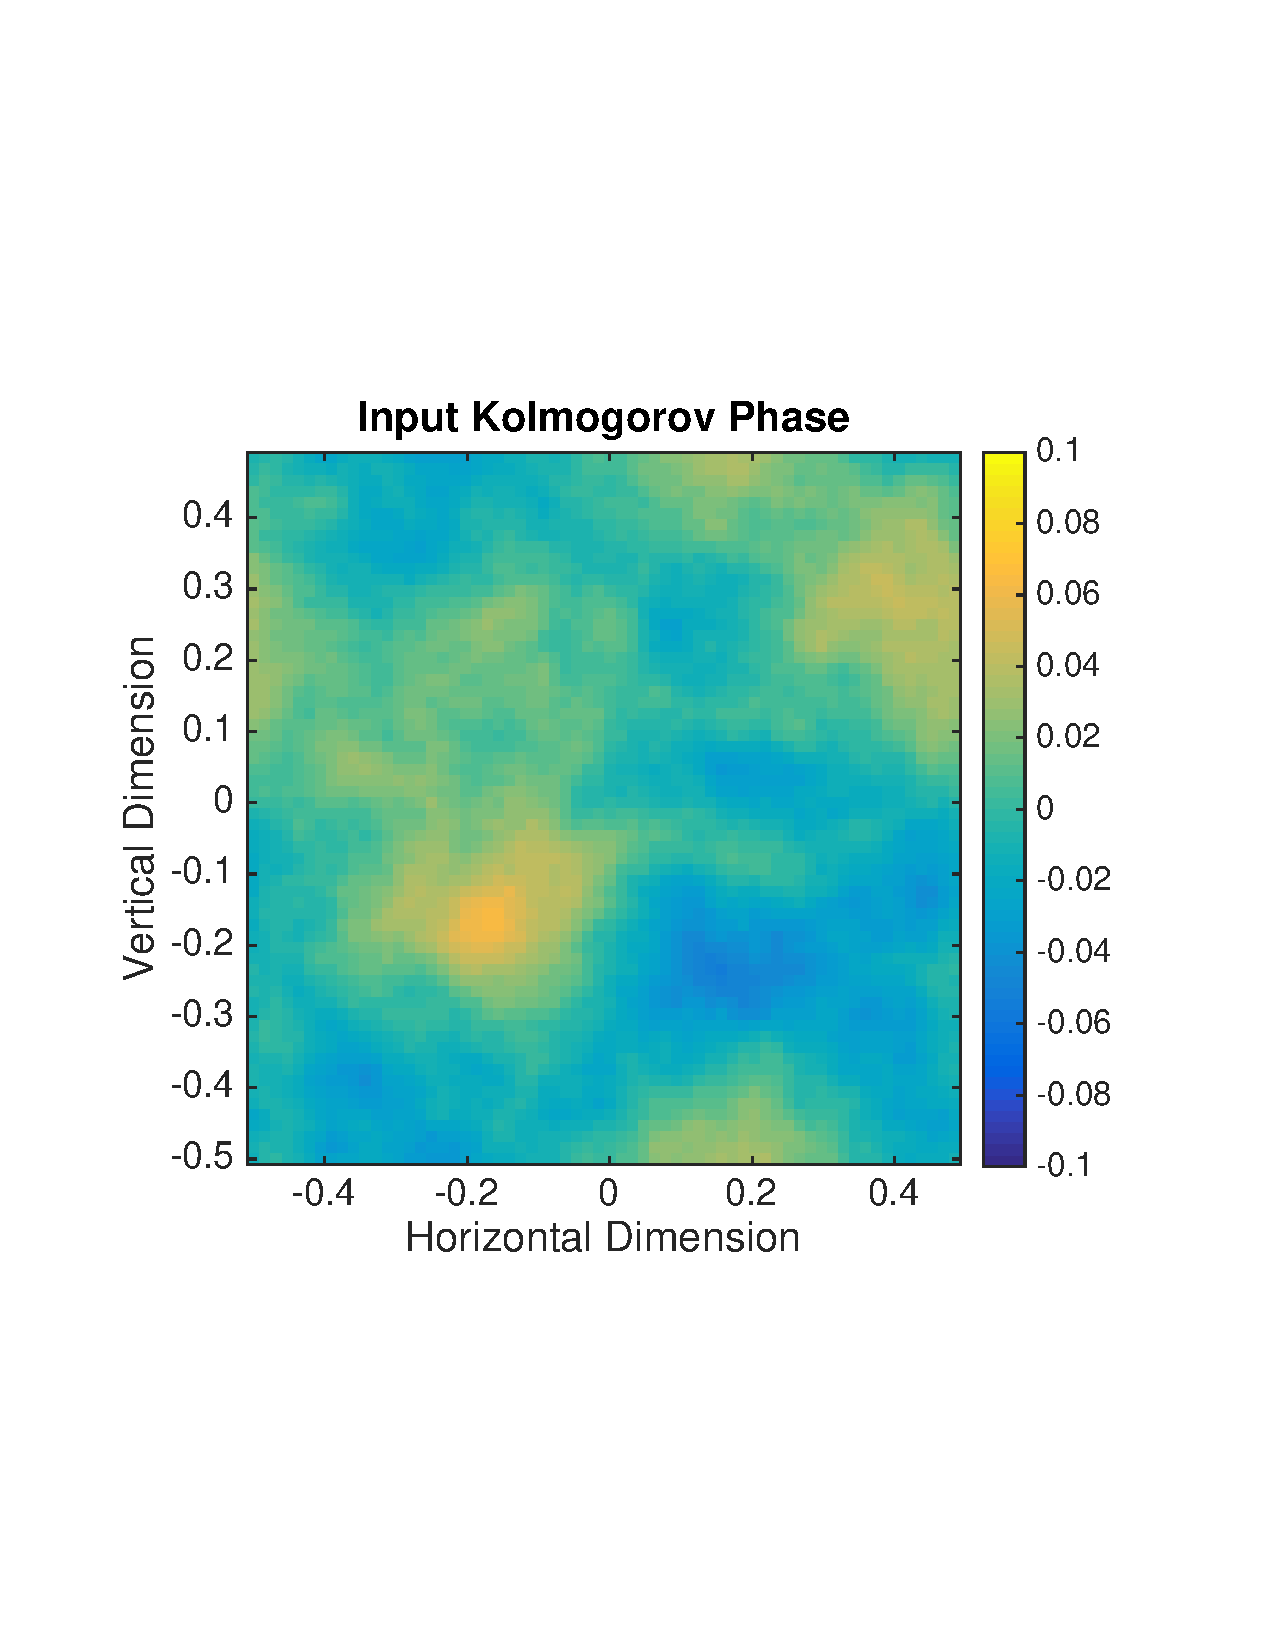
\includegraphics[trim = 0.8in 2.5in 1in 2.5in, clip, width = 1.8in]{kolmogorov.pdf}}
		\subfigure[]{\label{fig:bigfig_b}\includegraphics[trim = 0.8in 2.5in 1in 2.5in, clip, width = 1.8in]{DMapplied.pdf}}
		\subfigure[]{\label{fig:bigfig_c}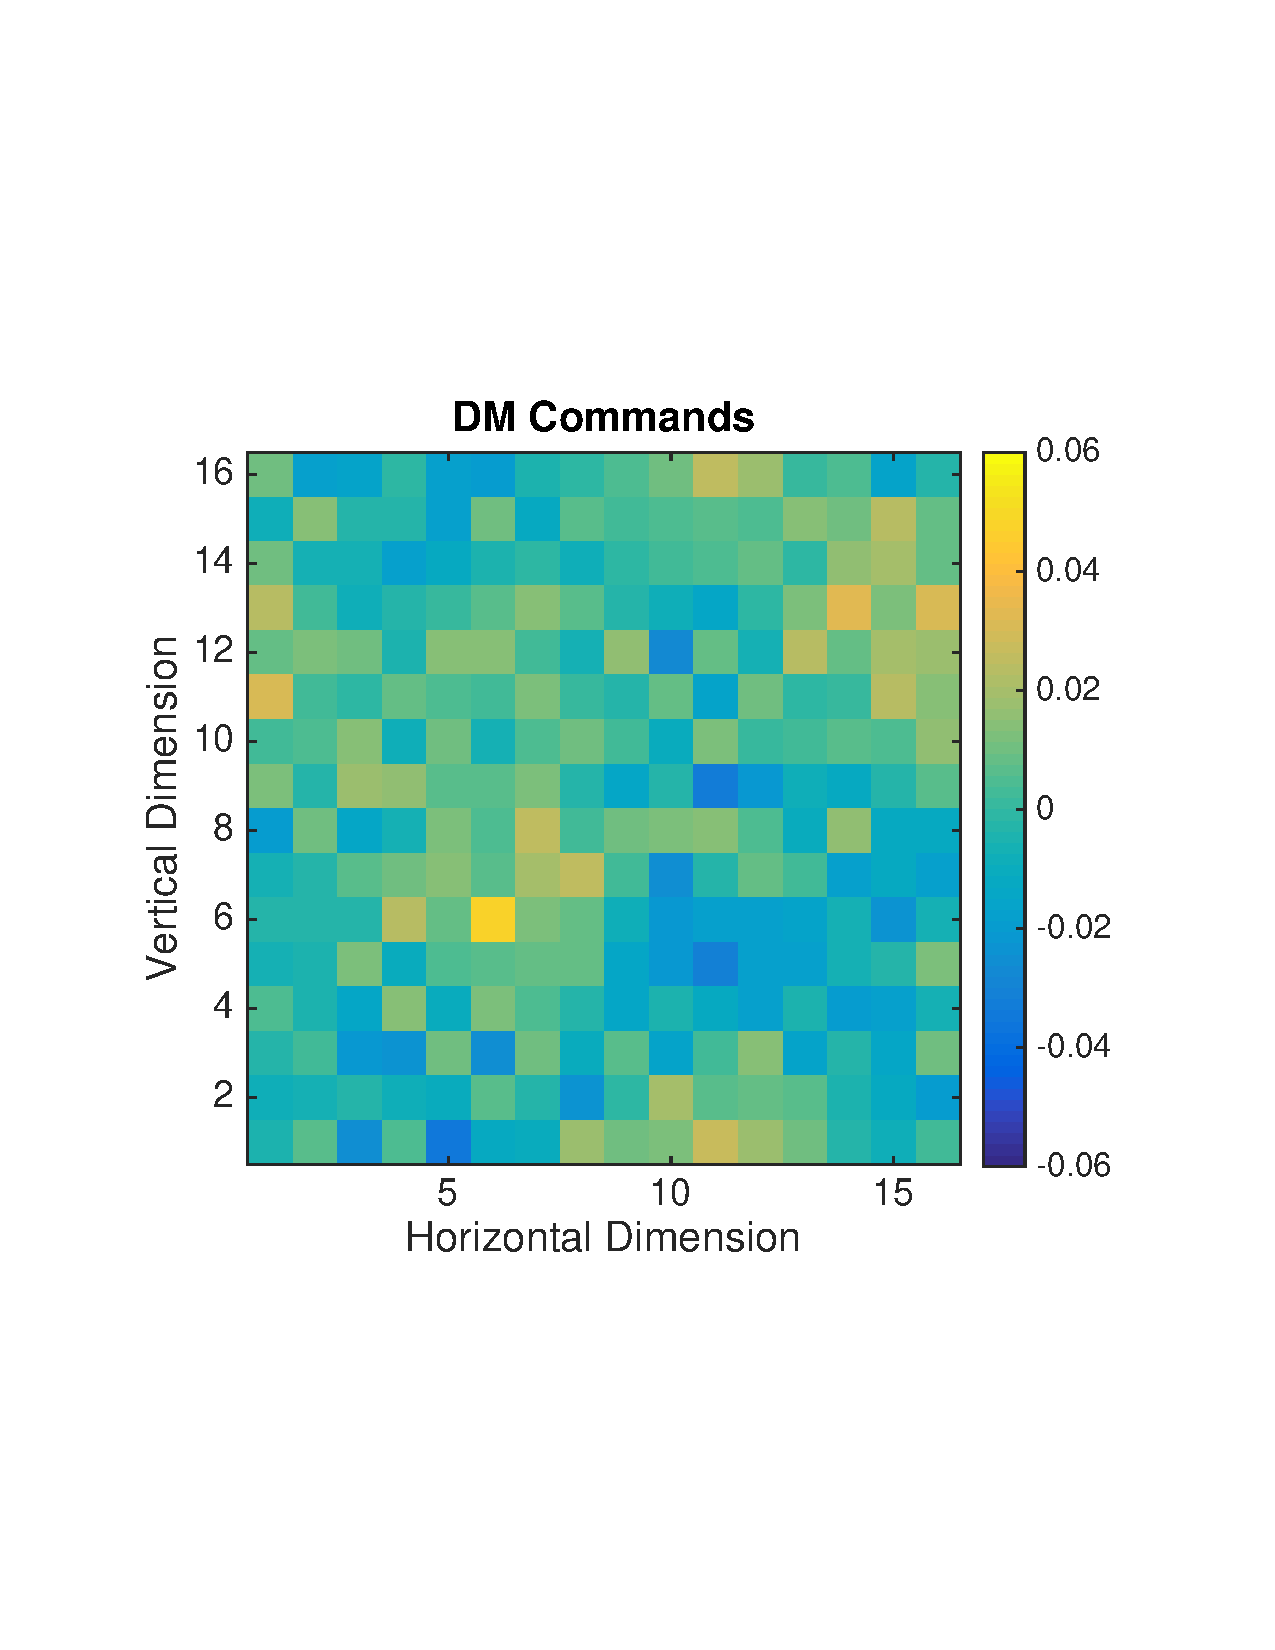
\includegraphics[trim = 0.8in 2.5in 1in 2.5in, clip, width = 1.8in]{DMcommands.pdf}}\\
		\subfigure[$\mbf{x}$]{\label{fig:bigfig_d}\includegraphics[trim = 0.8in 2.5in 1in 2.5in, clip, width = 1.8in]{truestate.pdf}}
		\subfigure[$\hat{\mbf{x}}(+)$]{\label{fig:bigfig_e}\includegraphics[trim = 0.8in 2.5in 1in 2.5in, clip, width = 1.8in]{updatedstateest.pdf}}
		\subfigure[$\mbf{x}-\hat{\mbf{x}}(+)$]{\label{fig:bigfig_f}\includegraphics[trim = 0.8in 2.5in 1in 2.5in, clip, width = 1.8in]{updatedstateresidual.pdf}}\\
		\subfigure[]{\label{fig:bigfig_g}\includegraphics[trim = 0.8in 2.5in 1in 2.5in, clip, width = 1.8in]{DMtrueshape.pdf}}
		\subfigure[]{\label{fig:bigfig_h}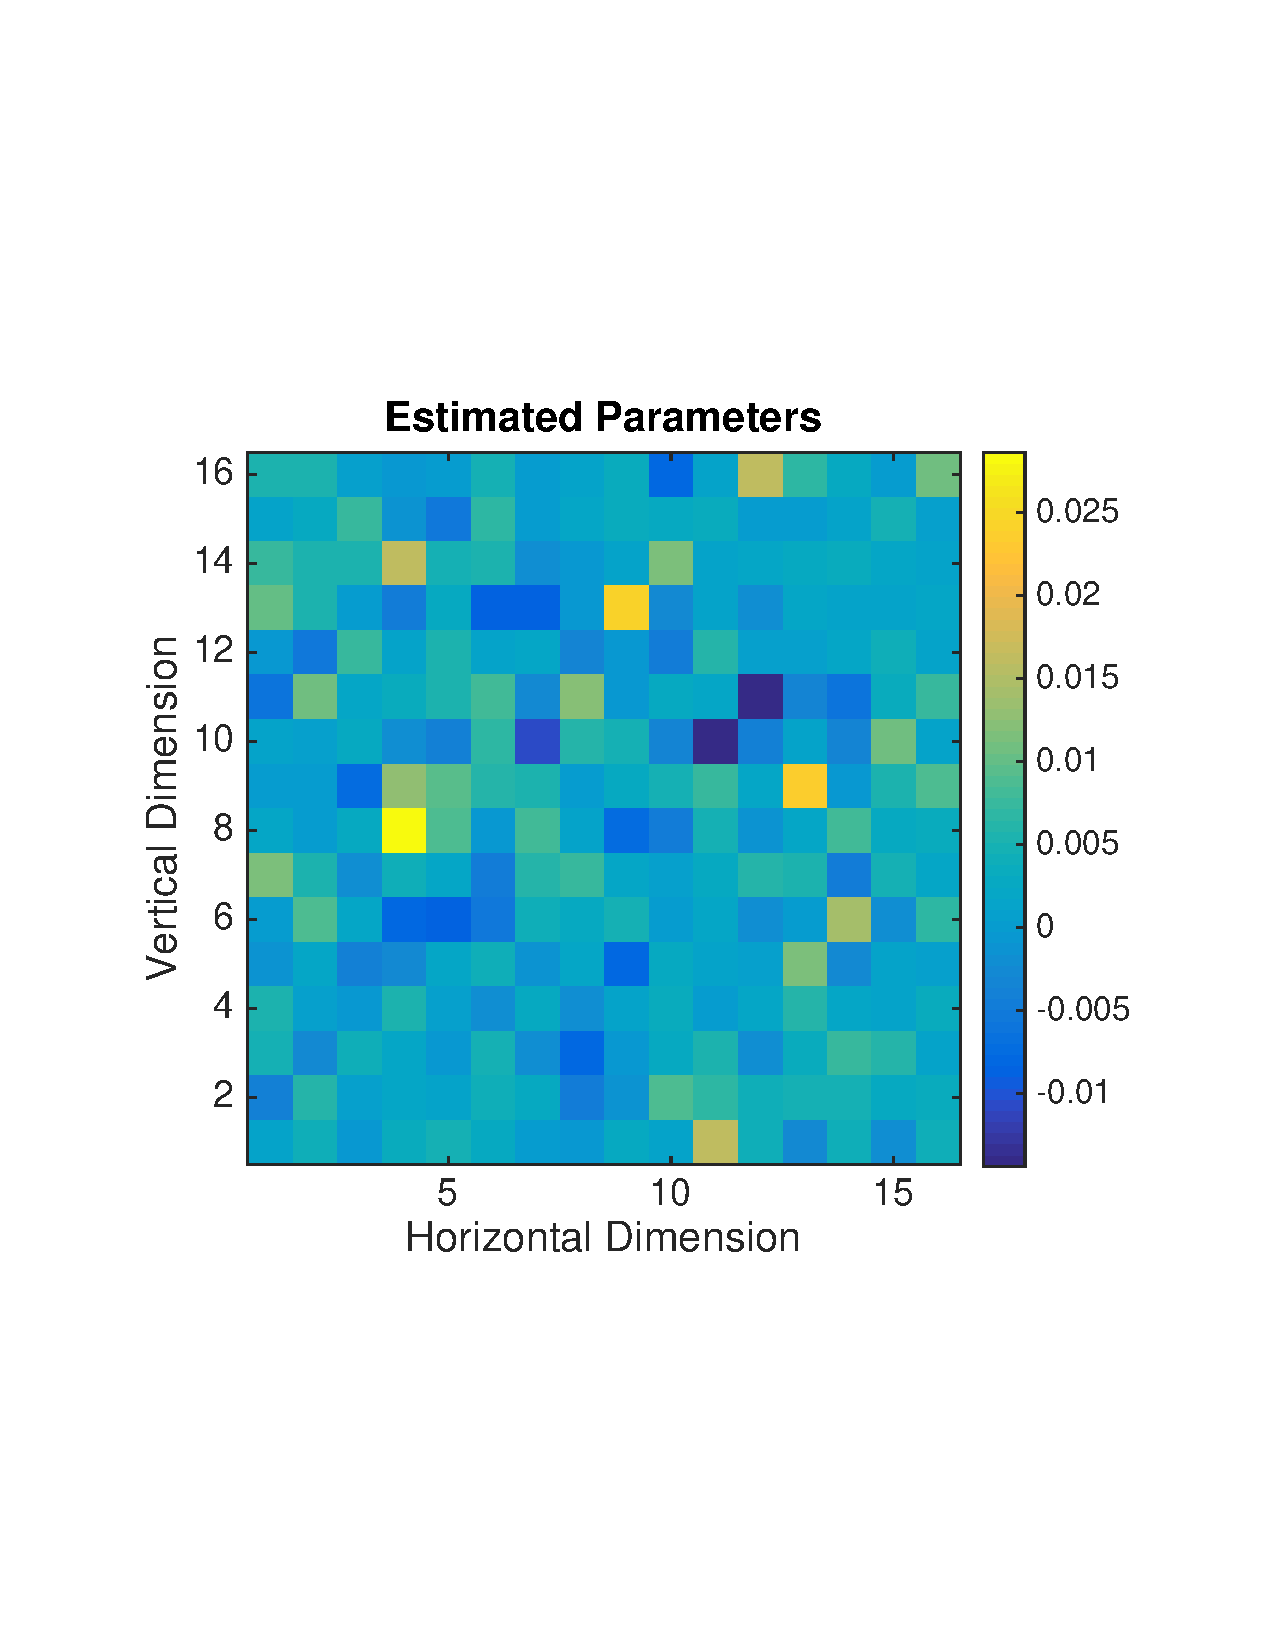
\includegraphics[trim = 0.8in 2.5in 1in 2.5in, clip, width = 1.8in]{params.pdf}}
		\subfigure[]{\label{fig:bigfig_i}\includegraphics[trim = 0.8in 2.5in 1in 2.5in, clip, width = 1.8in]{Imageplane.pdf}}
	\end{center}
\caption{Adaptive Kalman filter results after ten iterations.  The input Kolmogorov phase (a), the applied DM shape (b), and the corresponding actuator commands (c) are shown in the first row.  The state (d), final state estimate (e), and state residual (f) follow in the second row.  The imperfect true DM shape that results after all influence functions are given equal unit weight (g), the final parameter estimates (h), and the image (i) with final contrast of $\sim\!\!10^{-5.8}$ compose the third row. \label{fig:bigfig}}
\end{figure}

The final state, $\mbf{x}$, exhibits errors with spatial frequencies on the order of the actuator spacing; this is not a surprising result, as the phase conjugation method is fundamentally limited in the spatial frequencies of aberration that it can correct by the Nyquist limit corresponding to the actuator spacing.  The simulation was formatted in a way that the Kolmogorov input and true DM shapes would be truly random for each execution of ten iterations; performance varied little (qualitatively) from what is demonstrated here.  There is little qualitative evidence that the adaptive extended Kalman filter performs significantly better than the standard Kalman filter implemented without parameter estimation; upon tuning the magnitude of the FWHM variations in the true DM influence functions, when the variation is increased beyond a certain threshold so that convergence is not achieved, both algorithms diverge similarly.  The adaptive filter also appears to converge in a more smooth fashion, but not significantly so.  Although one could be convinced upon comparison of Figures \ref{fig:bigfig_g} and \ref{fig:bigfig_h} that the adaptive filter is attempting to conform to at least the largest of the DM shape variations, there is not good agreement between the estimated parameters and the true parameters.

\begin{figure}[h!]
\centering
\includegraphics[trim = 0.8in 2.5in 0.8in 2.5in, clip, width = 4in]{contrastcompare.pdf}
\caption{Comparison of typical achieved contrast between standard Kalman filter with unadjustable DM model and parameter-adaptive extended Kalman filter.}
\label{fig:contrastcompare}
\end{figure}

Several explanations for this lack of agreement can be made.  The observability of the FWHM of the Gaussian influence functions in the residual phase error was not calculated/tested; the control effect of the width of the influence function---as opposed to its gain---needs to be examined.  Furthermore, the nature of the dynamics could be chosen so as to elucidate better whether the parameter estimation is tracking the true value; one method would be to create a true DM model with parameters varying sinusoidally in magnitude, and examine the time evolution of the parameter estimates for corresponding sinusoidal behavior.  Perhaps a more accesible parameter would involve an estimation of the bias or nonlinearity of a MEMS DM response with the control input.  Improvements of this nature are currently being made which also implement an model of a MEMS DM rather than the influence functions chosen here \cite{Vogel2006}.

%%%%%%%%%%%%%%%%%%%%%%%%%%%%%%%%%%%%%%%%%%
\section{Conclusions and Final Remarks}\label{sec:conclusion}
An parameter-adaptive Kalman filter has been applied, in simulation, to the problem of wavefront control for high-contrast imaging.  A DM model based on Gaussian influence functions was linearized with respect to the width of the Gaussian functions, and these widths were taken to be the model parameters adjustable by the adaptive filter.  Application of both a standard estimator as well as an adaptive estimator to a ground-based wavefront control system with Kolmogorov turbulence input and a phase conjugation control scheme was simulated in closed loop; the goal of each routine was to drive the residual phase error to zero so as to create an image with high contrast.  The residual error and image contrast were used as metrics to compare the two estimators, which ran for ten iterations of the control loop.  The two estimators were shown to perform similarly, but this does not necessarily indicate the failure or infeasibility of parameter-adaptive estimation.  Choosing the widths of the influence function as the adjustable parameters may not have been the best choice for the filter, as it is not clear whether variations in these parameters are observable in the phase error.


%%%%%%%%%%%%%%%%%%%%%%%%%%%%%%%%%%%%%%%%%%%

\bibliographystyle{abbrv}
\bibliography{/Users/jamesmadison/Dropbox/BibTeX/FerroDM.bib}

\end{document}  